\chapter{AODV vs. DSDV}
\label{chap:aodvdsdv}

\section{Ejercicio 3.1}

\subsection{¿En qué instante se realiza la primera transmisión (de cualquier tipo de paquete) con AODV? ¿Y con DSDV?
¿Por qué?}

La primera transmisión de AODV se hace a los 10.002 segundos. En cambio, DSDV transmite el primer paquete a los 0.056 segundos.

La diferencia que hay es dado a que DSDV es un protocolo proactivo por lo que va actualizando cada poco tiempo las tablas de enrutamiento para así mantener la información fresca, en cambio AODV es un protocolo reactivo, solo manda paquetes cuando es necesario.

\section{Ejercicio 3.2}

\subsection{¿En qué instante recibe static2 el datagrama UdpBasicAppData-0 con AODV? ¿Y con DSDV? ¿Por qué?}

Con AODV static2 recibe el datagrama a los 11.4526 segundos, mientras que con DSDV lo recibe a los 10.0030 segundos. Esto ocurre porque en AODV los nodos tienen que ir actualizando la tabla de enrutamiento para poder encontrar la ruta y esto lleva un tiempo extra, en cambio en DSDV al tener todos los nodos sus tablas actualizadas, a la hora que querer establecer la ruta ya lo hace al instante.


\section{Ejercicio 3.3}

\subsection{¿Cuántos paquetes se pierden como consecuencia de la caída del nodo en AODV? ¿Y en DSDV? ¿A qué se
debe la diferencia? (Nota: para calcular el número de paquetes perdidos avanza hasta un instante posterior a la
caída en el que en ambos escenarios static2 vuelva a recibir datagramas y calcula la diferencia entre el número
de paquetes recibidos en static2 con y sin la caída del nodo).}

Para el caso de DSDV tuvimos que usar la semilla 65634 para poder ver con claridad la pérdida de paquetes y asi hacer la comparación.

Hemos hecho las simulaciones en ambos casos hasta los 22 segundos y en la tabla \ref{tabla1} se ven los resultados:

\begin{table}[H]
    \centering
    \begin{tabular}{|c|c|c|c|}
    \hline
    Protocolo & Sin fallo & Con fallo & \% pérdidas \\ \hline
      AODV    &   325     &   323     &     0.6\%   \\ \hline
      DSDV    &   254     &   156     &     38.5\%  \\ \hline
    \end{tabular}
    \caption{Tabla comparativa pérdida paquetes al caer un nodo}
    \label{tabla1}
\end{table}

Como vemos, en AODV la pérdida de paquetes es irrisorio con respecto a DSDV. Esto se debe a que en AODV, cuando un nodo detecta un fallo en la ruta, este envía un RERR a todos los nodos para informarlos del error por lo que se empieza a buscar inmediatamente otra ruta alternativa. En cambio en DSDV, cuando un nodo detecta una ruta inválida, no se genera otra ruta hasta que todos los nodos tengan su tabla de enrutamiento actualizada por lo que esto se traduce a una pérdida significativa de paquetes ya que tardan en actualizar sus tablas un cierto período de tiempo. 

\section{Ejercicio 3.4}

\subsection{Con la caída del nodo desactivada, simula AODV y DSDV durante 300 s (sim-time-limit). Muestra
capturas de los nodos estáticos a nivel de aplicación (doble click sobre el nodo) al final de la simulación. ¿Qué
porcentaje de los UdpBasicAppData enviados por static1 llega a static2? Explica los valores y las diferencias
observadas}

Primero vamos a ver lo que pasa en AODV, para eso vamos a fijarnos en las siguientes imágenes:

\begin{figure}[H]
    \centering
    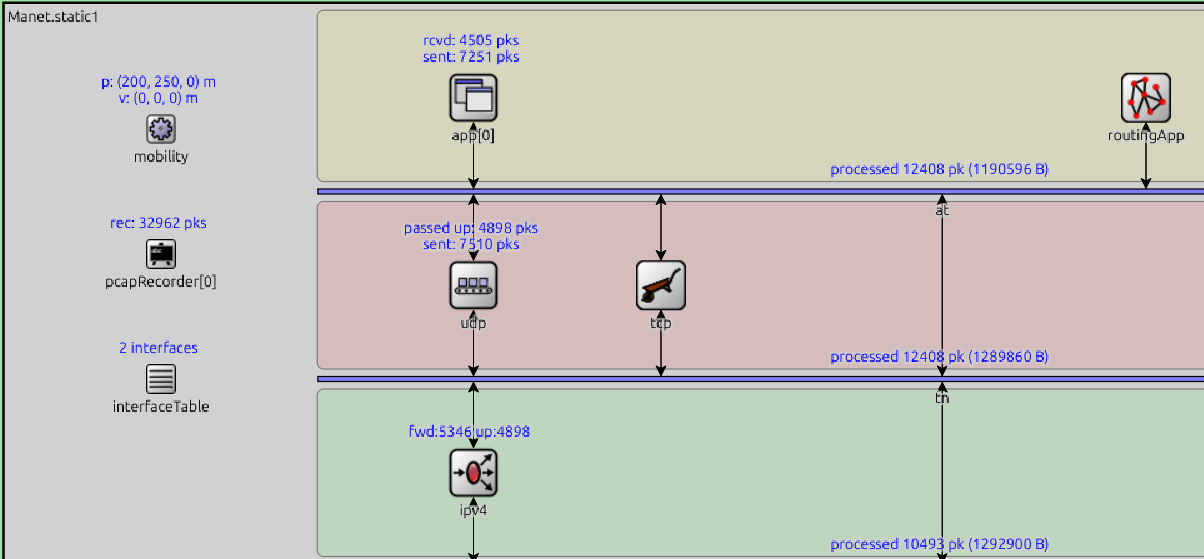
\includegraphics[width=155mm, scale=0.75]{imaxes/aodv_dsdv/ejercicio3_4_static1_aodv.png}
    \caption{Static1 a los 300s en AODV}
    \label{fig:ejer3_4_1}
\end{figure}

\begin{figure}[H]
    \centering
    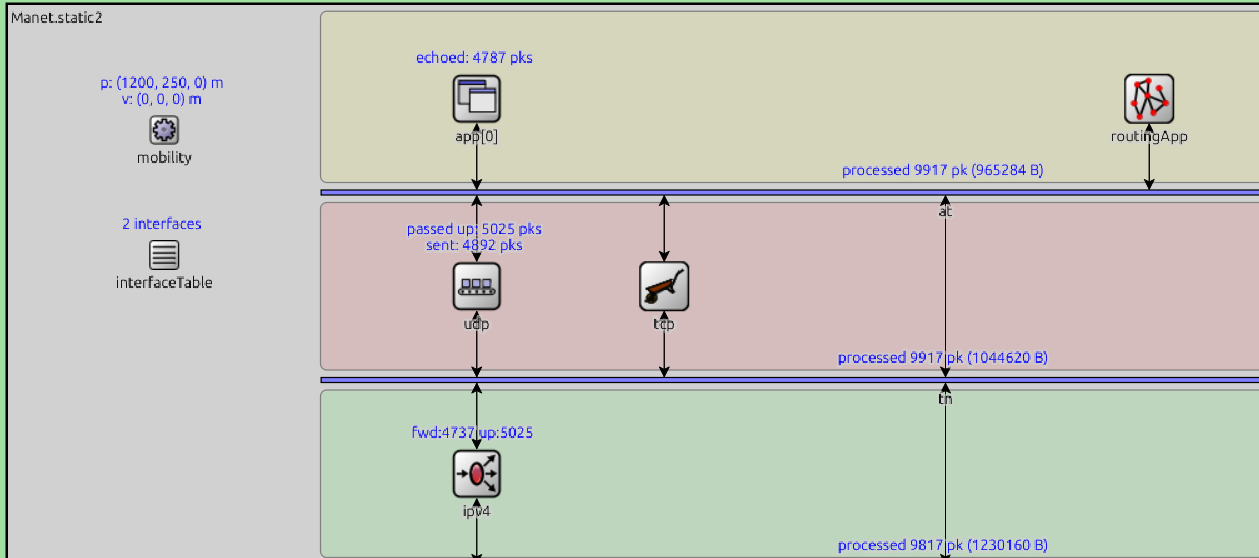
\includegraphics[width=155mm, scale=0.75]{imaxes/aodv_dsdv/ejercicio3_4_static2_aodv.png}
    \caption{Static2 a los 300s en AODV}
    \label{fig:ejer3_4_2}
\end{figure}

Como vemos, en la imagen \ref{fig:ejer3_4_1}, static1 manda 7251 paquetes y static2 recibe 4787 (imagen \ref{fig:ejer3_4_2}), por lo que se traduce a que a static2 le llega el 66\% de los paquetes.

Ahora vamos a ver lo que pasa en DSDV:

\begin{figure}[H]
    \centering
    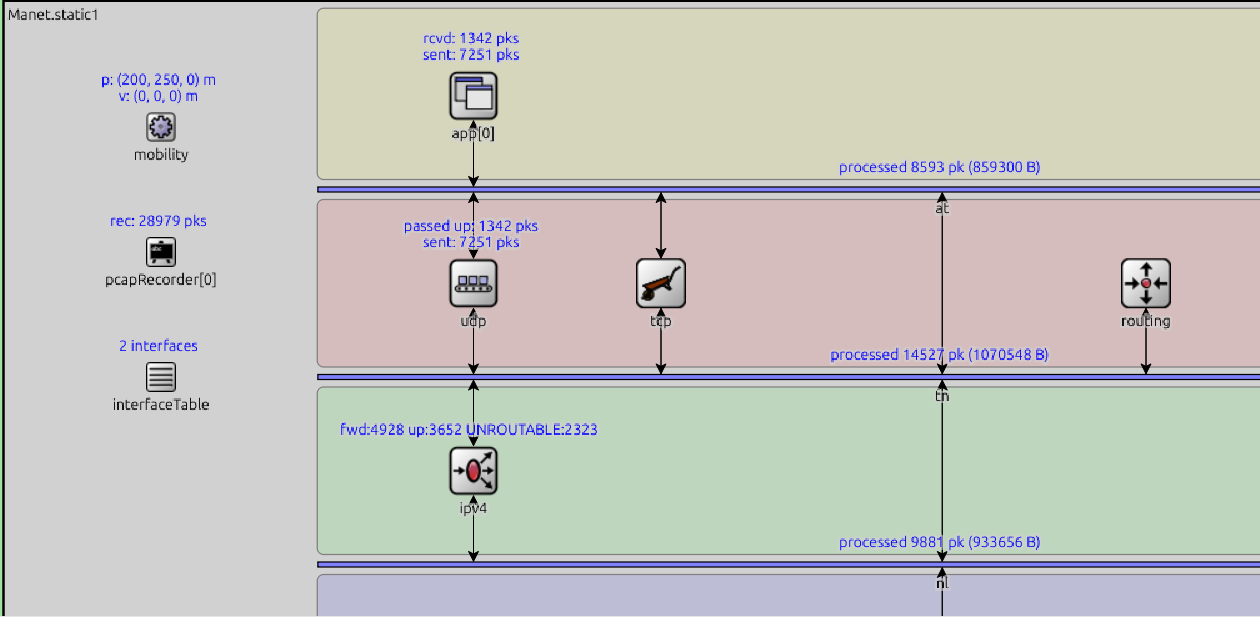
\includegraphics[width=155mm, scale=0.75]{imaxes/aodv_dsdv/ejercicio3_4_static1_dsdv.png}
    \caption{Static1 a los 300s en DSDV}
    \label{fig:ejer3_4_3}
\end{figure}

\begin{figure}[H]
    \centering
    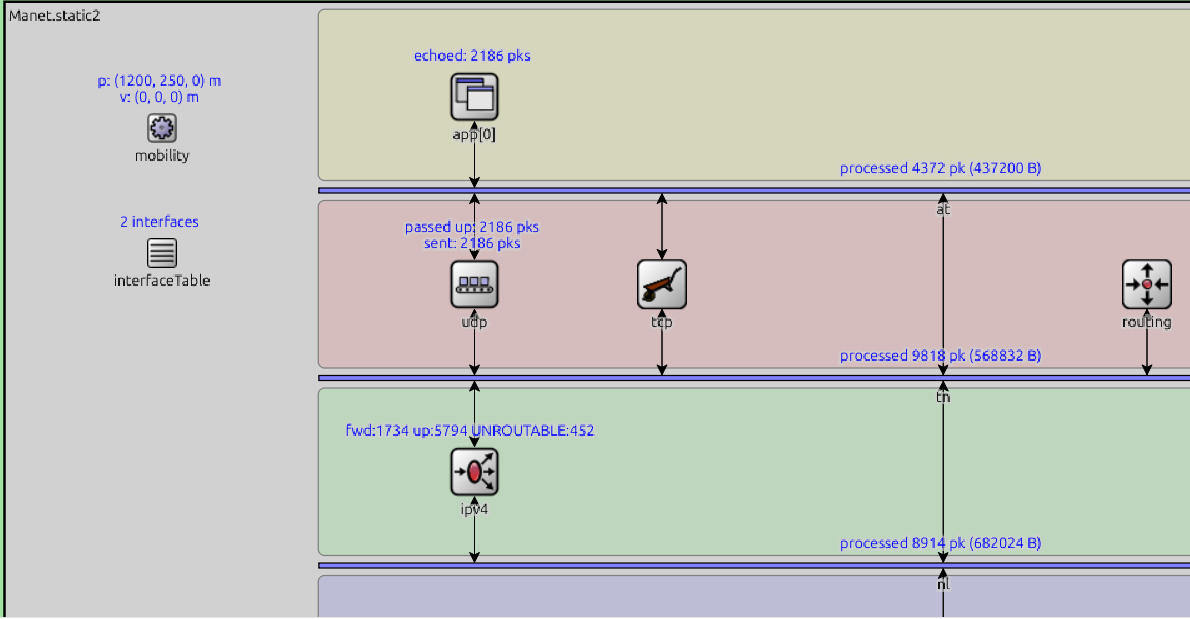
\includegraphics[width=155mm, scale=0.75]{imaxes/aodv_dsdv/ejercicio3_4_static2_dsdv.png}
    \caption{Static2 a los 300s en DSDV}
    \label{fig:ejer3_4_4}
\end{figure}

Si vemos la imagen \ref{fig:ejer3_4_3}, static1 manda 7251, mientras que a static2 le llegan 2186 (ver imagen \ref{fig:ejer3_4_4}), por lo que solamente le llega a static2 el 30\%.

La diferencia que hay entre AODV y DSDV es muy grande, concretamente DSDV pierde el doble de los paquetes con respeto AODV. Esto se debe a la constante actualización de las tablas de enrutamiento que hay en DSDV, por lo que cambia constantemente de ruta, mientras que en AODV cuando detecta una ruta, se mantiene todo el tiempo activa hasta que no sea válida. Además en DSDV cuando se cambia de ruta o deja de ser válida, tiene que volver a hacer el proceso de reconstrucción y esto se traduce en un período de tiempo que static2 no recibe ningún paquete de static1. 


\section{Ejercicio 3.5}

\subsection{¿Qué porcentaje de los paquetes devueltos por static2 llegan a static1? Explica los valores y las diferencias
observadas.}

Para el caso de AODV, static2 hace echo de los 4787 paquetes que recibe y static1 recibe 4505 paquetes (imagen \ref{fig:ejer3_4_1}), por lo que esto lleva a que static1 recibe el 94\% de los paquetes que le manda static2.

En DSDV, static2 manda 2186 paquetes y static1 recibe 1342 paquetes (imagen \ref{fig:ejer3_4_3}), por lo que se traduce a que static1 recibe el 61\% de los paquetes mandados por static2. 

La diferencia que hay entre AODV y DSDV es dado a como funciona cada protocolo. AODV por cada RREQ que se manda entre los nodos, hay un RREP haciendo la ruta inversa por por la misma ruta que se ha establecido de ida, por lo que es más difícil de que haya pérdida de paquetes. En cambio en DSDV al no haber un control en la ruta inversa, si algún nodo no es capaz de poder devolver el paquete, se pierde entonces hasta que tenga una ruta de vuelta actualizada/disponible. También hay que destacar que en DSDV hay una mayor congestión en el tráfico por lo que se puede provocar colisiones y sobrecargas.